% !TEX root = ../thesis.tex
\chapter{Approach}

% **************************** Define Graphics Path **************************
\ifpdf
\graphicspath{{Chapter3/Figs/Raster/}{Chapter3/Figs/PDF/}{Chapter3/Figs/}}
\else
\graphicspath{{Chapter3/Figs/Vector/}{Chapter3/Figs/}}
\fi

\section{Introduction}

Despite the importance of crowd monitoring in mass gathering events, the literature review in the previous chapter is able to identify several gaps in the research, especially in crowd modelling. Most state-of-art crowd monitoring techniques do not incorporate a typology to distinguish different types of crowd. In other words, no explicit type of crowd is defined in those approaches.

say something more about crowd modelling

conclude with the need of a crowd monitoring framework

\section{An Overview of the Crowd Monitoring Framework}

In this project, we propose the crowd monitoring framework for emergency management in mass gatherings. The objectives of the framework are: 
\begin{inparaenum}[i)]
\item to incorporate more sources of contextual data;
\item to classify a crowd into different crowd types;
\item to propose a set of crowd attributes and describe a crowd type under those attributes
\end{inparaenum}.

To achieve those objectives, as can be seen in Figure \ref{fig:frameworkOverview} the framework consists of three layers:
\begin{inparaenum}[i)]
\item Context data to handle different sources of information;
\item Crowd model to analyse the context data and classify type of a crowd;
\item Crowd monitoring to detect the dangerous crowd types in real time
\end{inparaenum}.

\begin{figure}[htbp!] 
\centering    
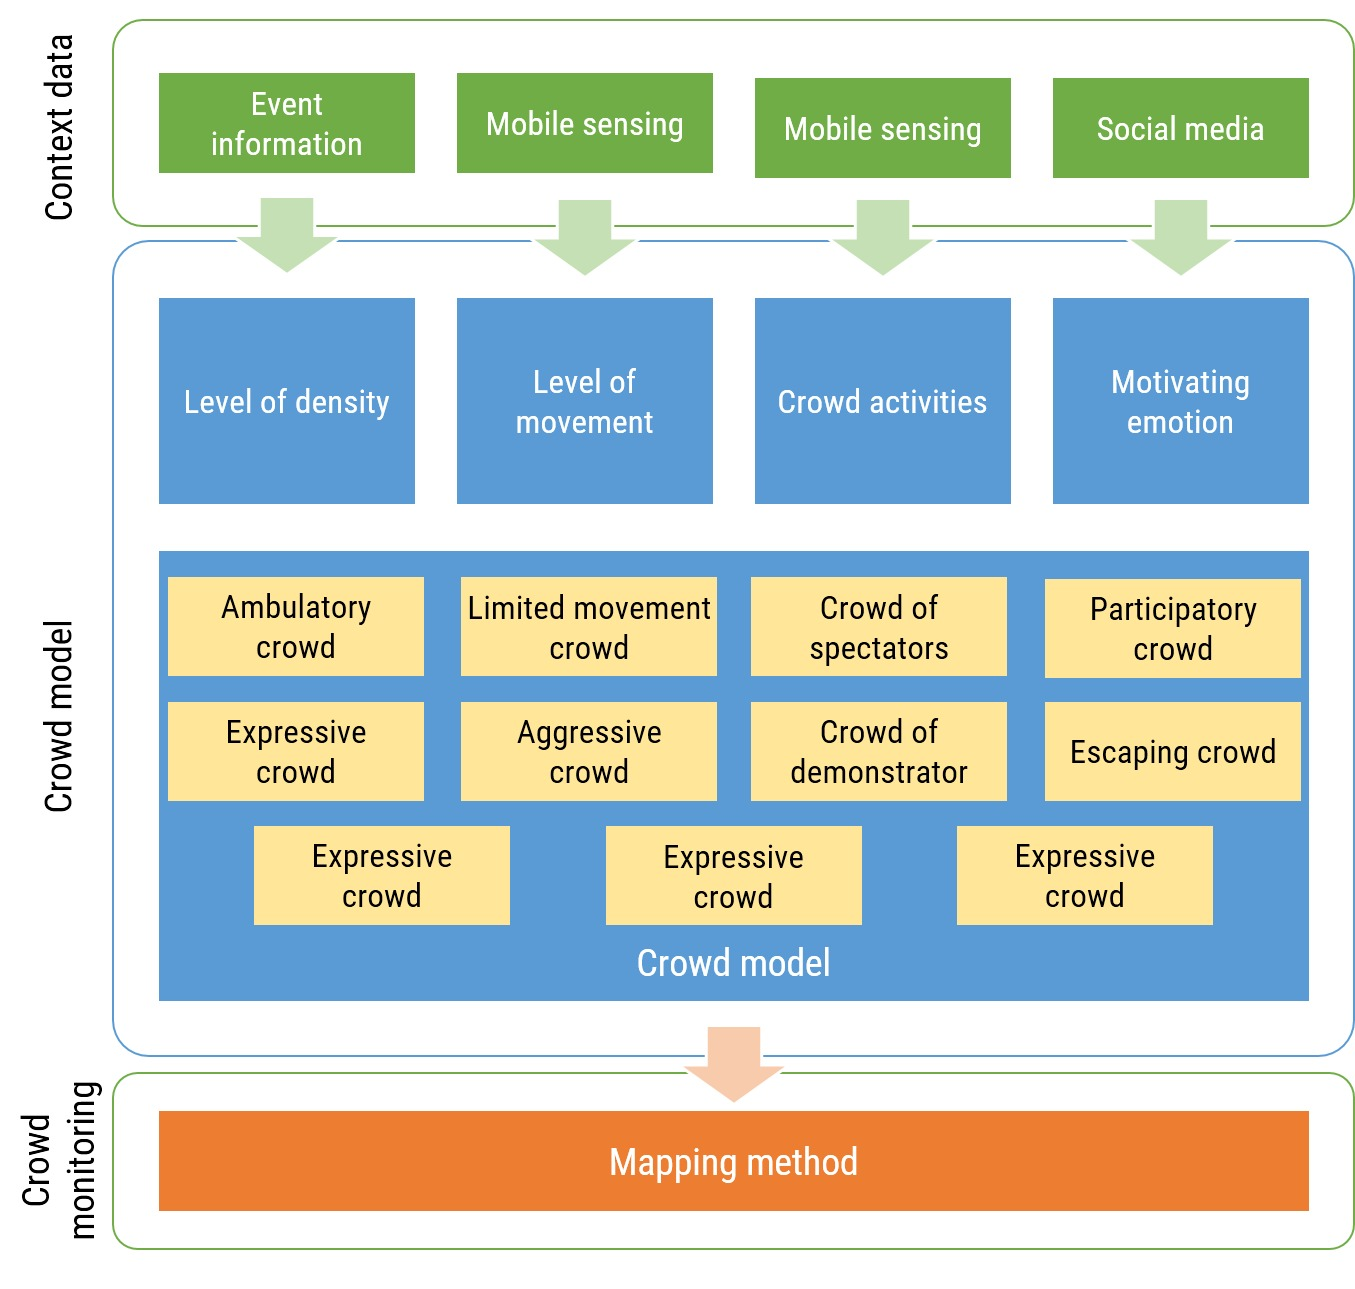
\includegraphics[width=1.0\textwidth]{FrameworkOverview}
\caption{An overview of the crowd monitoring framework using social media analysis}
\label{fig:frameworkOverview}
\end{figure}

Each component will be discussed further in the sections below.

\section{Social Media}
Social media is the generic term referring to a wide range of Internet based tools that enable user to create and share information. These tools include social network services such as Facebook and Twitter, Internet forums and channels. Among these tools, Twitter is the most common social media used in researches because of its large volume of users and its public API making the data highly accessible.

\section{Emotion Model}

We use Plutchik model

\section{Emotion Analysis of Social Media}

We can detect the dominating emotion from a tweet using a bag of word approach.

We then apply histogram with a specific time interval to measure the frequency of each emotion during that time frame.

\section{Crowd Model}

We use Berlonghi model

\section{Emotion - Crowd Type Mapping Model}

Table \ref{table:mappingEmotionCrowdType} presents our proposal for the mapping between each crowd type and eight basic emotions.
\begin{table}
\caption{Mapping between crowd types and emotions}
\label{table:mappingEmotionCrowdType}
\begin{tabular}{|p{2cm}|p{1.2cm}|p{1.2cm}|p{1.2cm}|p{1.2cm}|p{1.2cm}|p{1.2cm}|p{1.2cm}|p{1.2cm}|}
\hline
\textbf{Crowd type}	& \textbf{Anger}	& \textbf{Anticipation}	& \textbf{Joy} 	& \textbf{Trust}	& \textbf{Fear}	& \textbf{Surprise}	& \textbf{Sadness}	& \textbf{Disgust}	\\
\hline
Ambulatory			& low 				& medium				& medium		& medium			& low 			& low 				& medium			& low 		\\
\hline
Limited movement	& medium			& medium				& low 			& low 				& low 			& low 				& medium			& medium	\\
\hline
Spectator			& low 				& medium				& medium		& medium 			& low 			& medium			& low 				& low 		\\
\hline
Participatory		& low 				& medium				& medium		& medium			& low 			& low 				& low 				& low 		\\
\hline
Aggressive			& medium			& low 					& low 			& low 				& low 			& low 				& low 				& medium	\\
\hline
Demonstrator		& medium			& low 					& low 			& low 				& low 			& low 				& medium			& medium	\\
\hline
Escaping			& low 				& low 					& low 			& low 				& medium		& medium			& low 				& low 		\\
\hline
Dense				& medium			& low 					& low 			& low 				& medium		& medium			& low 				& medium	\\
\hline
Rushing				& medium			& low 					& low 			& low 				& low 			& low 				& low 				& medium	\\
\hline
Violent				& medium			& low 					& low 			& low 				& low 			& low 				& low 				& medium	\\
\hline
\end{tabular}
\end{table}

\section{Rule Based Reasoning}

\subsection{Fuzzifier}
We convert the numerical values of the frequency of appearance of an emotion into linguistic label: low, medium and high by applying following rules

if the value is below the low threshold of that emotion then the label is low
if the value is above the low threshold and below the high threshold then the label is medium
if the value is above the high threshold then the label is high

\subsection{Rule Repository}

list 11 rules here for 11 crowd types

\subsection{Inference Engine}

Fuzzy rule here and the mathematical formula here

\subsection{Output Processor}

the output is a vector of each crowd and its weight

\section{Conclusion}